\FloatBarrier
\subsubsection{Multivibrador astable}

La tabla \ref{tab:resultados-multivibrador-astable} muestra las mediciones del multivibrador astable.

\begin{table}[ht]
\centering
\begin{tabular}{|c|c|c|c|c|c|c|c|}
\hline
\(V_c\) & \(\Delta V_c\) & \(V_o\) & \(\Delta V_o\) & \(T\) & \(\Delta T\) & \(f\) & \(\Delta f\) \\ \hline
2.80 & 0.20 & 9.00 & 1.00 & 0.00023 & 0.00001 & 4347.826087 & \\ \hline
\end{tabular}
\caption{Mediciones del multivibrador astable.}
\label{tab:resultados-multivibrador-astable}
\end{table}

\begin{ilustracion}[ht]
    \centering
    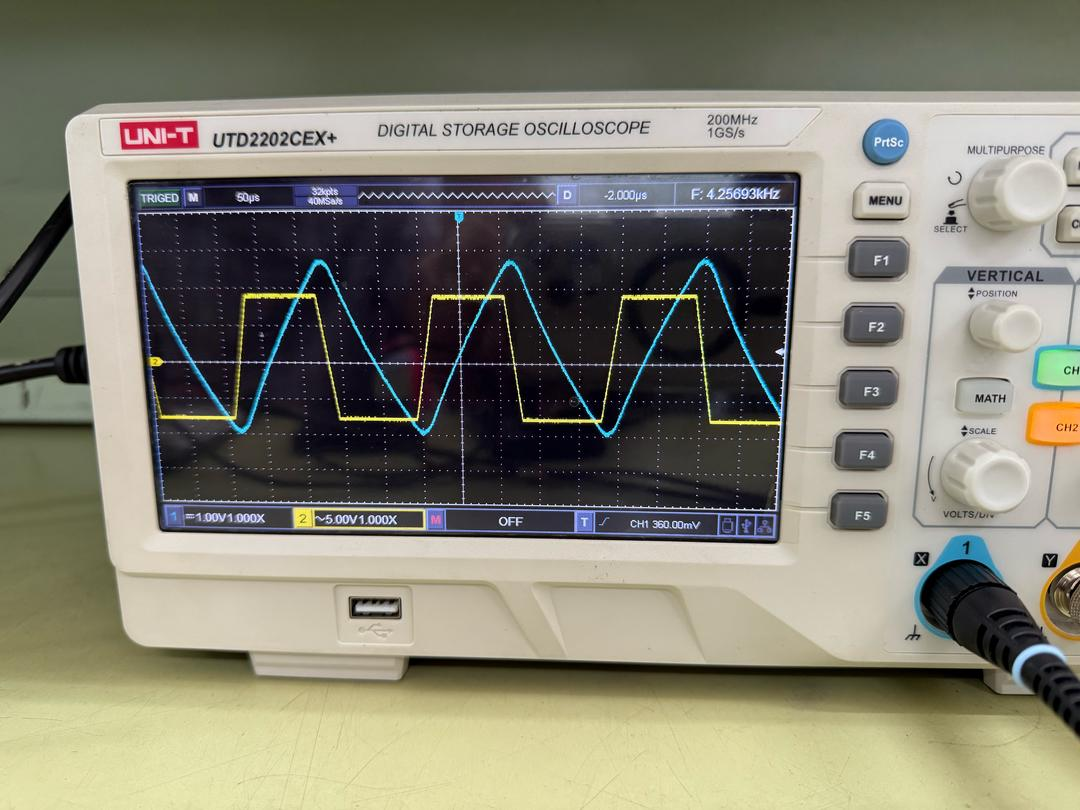
\includegraphics[width=0.6\textwidth]{resultados/astable-salida.jpg}
    \caption{Medición de voltajes del multivibrador astable (canal 1 $V_o$, canal 2 $V_c$).}
    \label{fig:multivibrador-astable-salida}
\end{ilustracion}

\subsubsection{Multivibrador monostable}

La tabla \ref{tab:resultados-multivibrador-monostable} muestra las mediciones DC del multivibrador monoestable antes de conectar el generador. $V_c$ es el voltaje en el condensador $C_6$ y $V_p$ es el voltaje en la salida del amplificador operacional.

\begin{table}[ht]
\centering
\begin{tabular}{|c|c|c|c|}
\hline
\(V_c\) & \(\Delta V_c\) & \(V_p\) & \(\Delta V_p\) \\ \hline
3.00 & 0.20 & 5.20 & 0.40 \\ \hline
\end{tabular}
\caption{Mediciones voltaje DC del multivibrador monoestable.}
\label{tab:resultados-multivibrador-monostable}
\end{table}

La ilustración \ref{ilus:multivibrador-monostable-salida} muestra la tensión en el condensador y el voltaje del generador con un periodo de 13ms y un duty cycle de 90\%.

\begin{ilustracion}
    \centering
    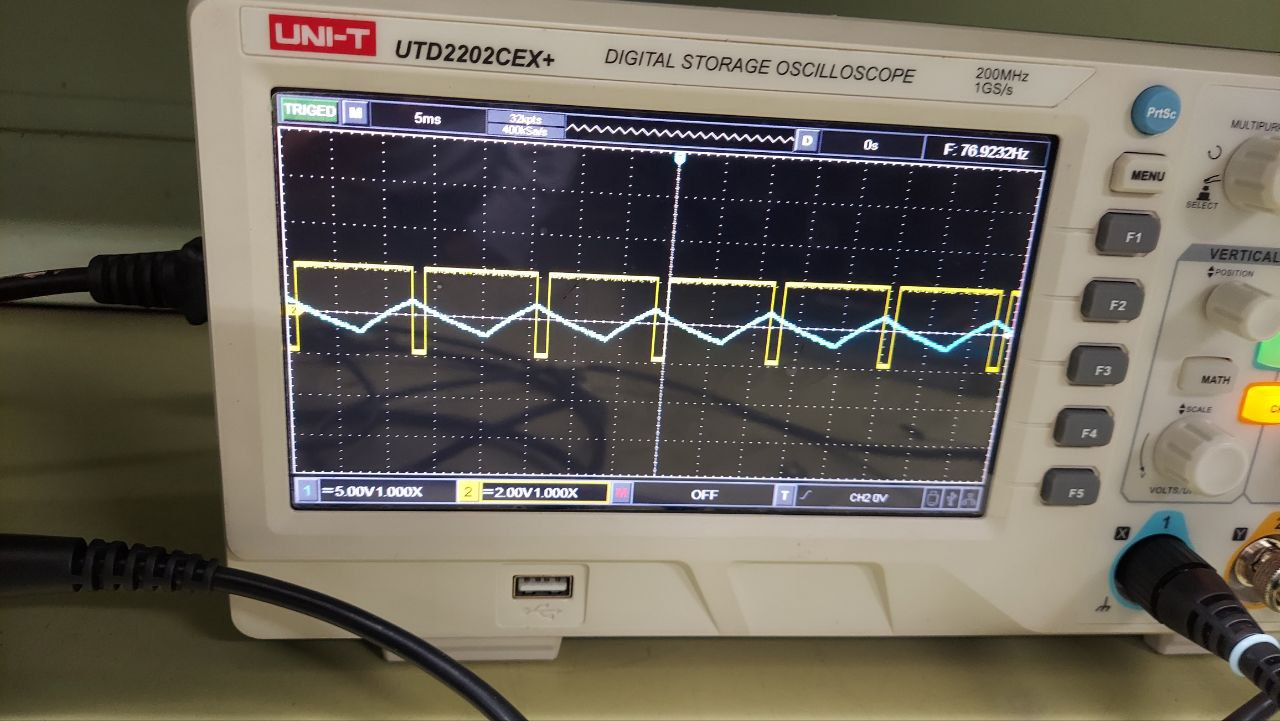
\includegraphics[width=0.6\textwidth]{resultados/monostable-90duty.png}
    \caption{Medición de voltajes del multivibrador monoestable (canal 1 $V_c$, canal 2 $V_c$). con un duty cycle del 90\% y T=13ms.}
    \label{ilus:multivibrador-monostable-salida}
\end{ilustracion}

\begin{ilustracion}
    \centering
    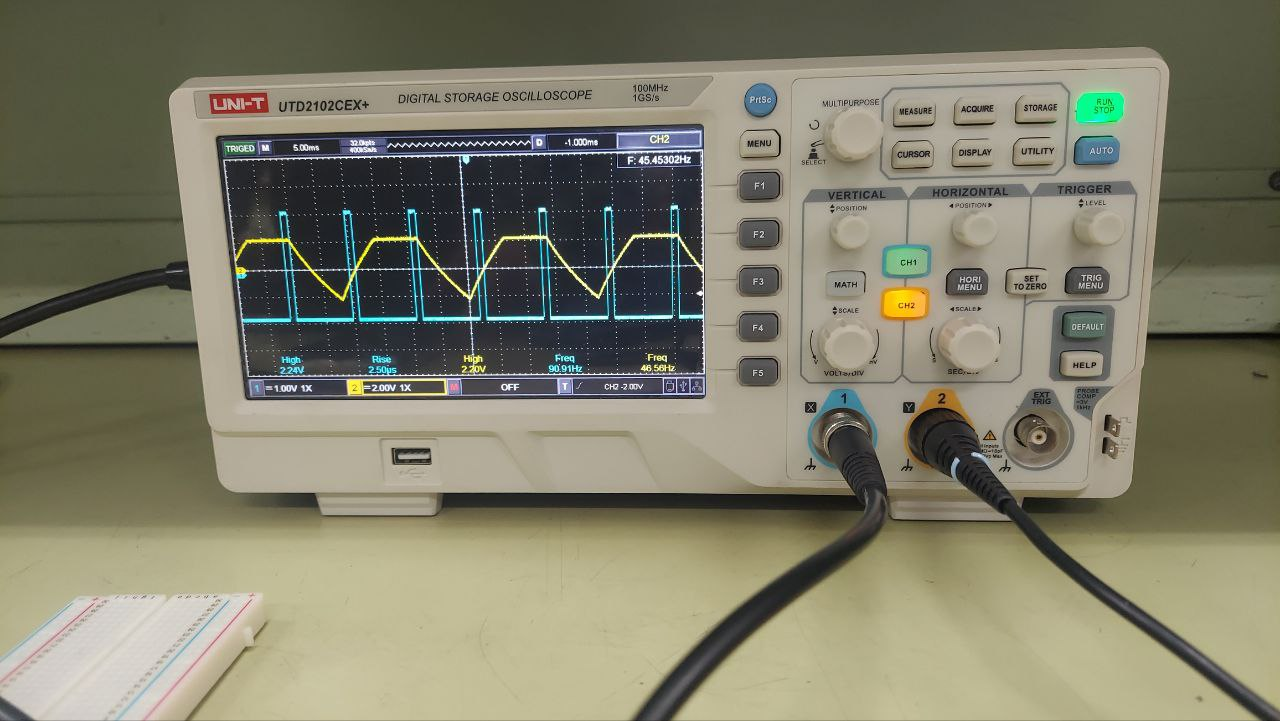
\includegraphics[width=0.6\textwidth]{resultados/monostable-11ms.png}
    \caption{Medición de voltajes del multivibrador monoestable (canal 1 $V_c$, canal 2 $V_c$). con un duty cycle del 10\% y T=11ms.}
    \label{ilus:multivibrador-monostable-salida-11ms}
\end{ilustracion}

\begin{ilustracion}
    \centering
    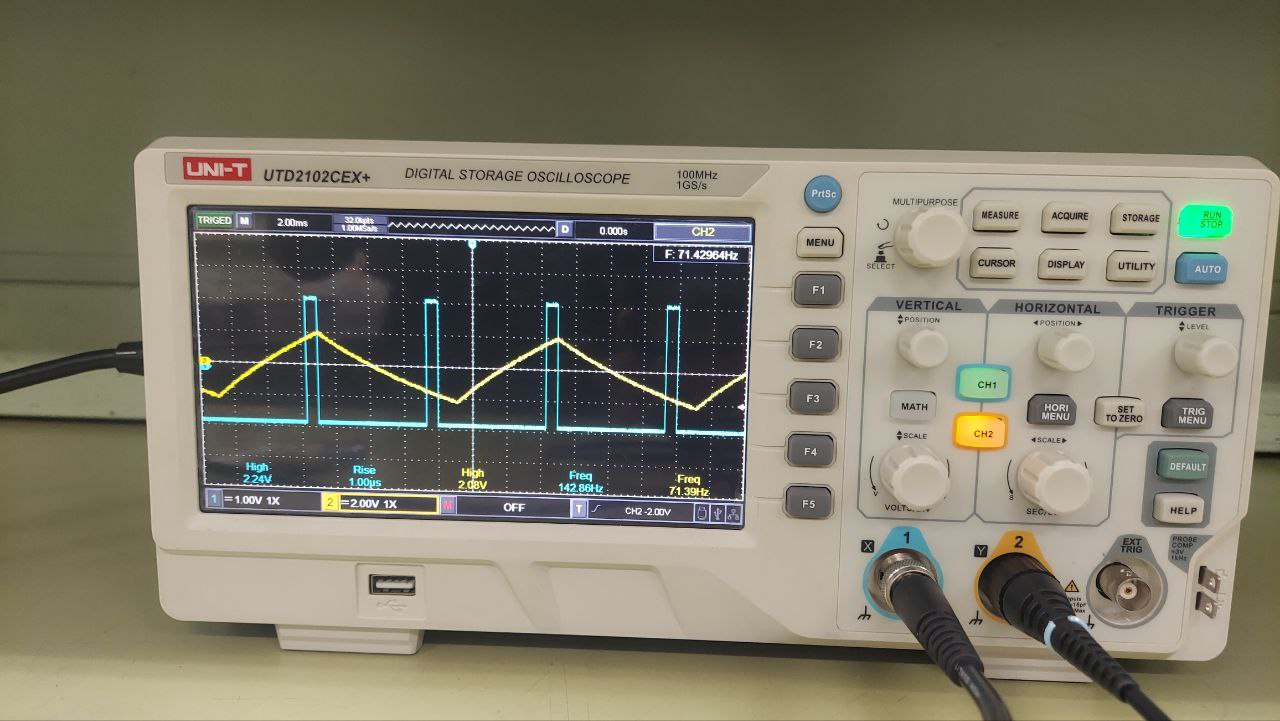
\includegraphics[width=0.6\textwidth]{resultados/monostable-7ms.png}
    \caption{Medición de voltajes del multivibrador monoestable (canal 1 $V_c$, canal 2 $V_c$). con un duty cycle del 10\% y T=7ms.}
    \label{ilus:multivibrador-monostable-salida-7ms}
\end{ilustracion}

La tabla \ref{tab:resultados-multivibrador-monostable-2} muestra las mediciones adicionales del multivibrador monoestable a partir de la ilustración \ref{ilus:multivibrador-monostable-salida-7ms}.

\begin{table}[ht]
\centering
\begin{tabular}{|c|c|c|c|}
\hline
\(V_c\) [V] & \(\Delta V_c\) [V] & \(T\) [ms] & \(\Delta T\) [ms]\\ \hline
2.00 & 0.40 & 14.00 & 0.40 \\ \hline
\end{tabular}
\caption{Mediciones del multivibrador monoestable con el generador conectado.}
\label{tab:resultados-multivibrador-monostable-2}
\end{table}

\begin{table}[ht]
\centering
\begin{tabular}{|c|c|c|c|}
\hline
\(T\) [ms] & \(\Delta T\) [ms] & Valor teórico [ms] & Error \% \\ \hline
14 & 0.4 & 10 & 40 \\ \hline
\end{tabular}
\caption{Comparación de mediciones y valores teóricos del multivibrador monoestable.}
\label{tab:comparacion-multivibrador-monostable}
\end{table}